\documentclass[a4paper,12pt]{article}
\usepackage[utf8]{inputenc}
\usepackage[german]{babel}
\usepackage{amsmath}
\usepackage{amssymb}
\usepackage{amsthm}
\usepackage{geometry}
\usepackage{graphicx}
\usepackage[hidelinks]{hyperref}
\usepackage{listings}
\usepackage{xcolor}
\usepackage{enumitem}
\usepackage[protrusion=true,expansion=false]{microtype}
\usepackage{csquotes}
\usepackage{booktabs}
\usepackage{caption}

\geometry{margin=2.5cm}
\emergencystretch=2em

\theoremstyle{definition}
\newtheorem{definition}{Definition}
\newtheorem{beispiel}{Beispiel}
\newtheorem{satz}{Satz}
\newtheorem{lemma}{Lemma}
\newtheorem{bemerkung}{Bemerkung}
\newtheorem{korollar}{Korollar}
\newtheorem{these}{These}

\setlist[itemize,1]{label=--}

% ---------- Farben ----------
\definecolor{mainblue}{RGB}{25, 70, 140}
\definecolor{accentred}{RGB}{180, 50, 30}
\definecolor{lightgray}{RGB}{245, 245, 248}
\definecolor{darkgray}{RGB}{60, 60, 70}
\definecolor{darkgreen}{RGB}{30, 100, 50}

\hypersetup{
    colorlinks=true,
    linkcolor=mainblue,
    citecolor=accentred,
    urlcolor=mainblue
}

% Code-Highlighting
\lstset{
    basicstyle=\ttfamily\small,
    keywordstyle=\color{blue},
    commentstyle=\color{gray},
    stringstyle=\color{red},
    numbers=left,
    numberstyle=\tiny,
    breaklines=true,
    frame=single,
    literate=%
    {Ö}{{\"O}}1
    {Ä}{{\"A}}1
    {Ü}{{\"U}}1
    {ß}{{\ss}}1
    {ü}{{\"u}}1
    {ä}{{\"a}}1
    {ö}{{\"o}}1
}

\title{\textbf{Grenzen der menschlichen Erforschung:}\\[0.4em]
\large Erde, Sonne, Mond und Meer als primäre Erkenntnisräume\\
des Menschen gegenüber galaktischen und kosmologischen Skalen}
\author{Stephan Epp}
\date{23. Juni 2026}

\begin{document}

\maketitle

\bigskip

\begin{center}
\begin{minipage}{0.88\textwidth}
\itshape
\small
\enquote{Die Galaxien sind für mich völlig übertrieben. Allein der Gedanke daran,
sie zu erforschen, grenzt an die allergrößte Verlorenheit, die es je für den
Menschen gab. Die Sonne, der Mond, die Erde und das Meer sind so viele Extreme
für das Leben auf dieser Erde. Der Mensch hat immer sein Leben lang daran zu tun,
wenn er sich Gedanken machen will, über diese Extreme für das Leben nachzudenken
und sie zu erforschen. Wer darüber hinausgeht und weiter in die Galaxien gehen
will, der ist nicht mehr ganz dicht und sieht nicht, wo er eigentlich herkommt.}

\medskip

\enquote{Das Beschäftigen mit den Galaxien oder dem Universum zieht ins Verderben.
Noch näher und noch schlimmer ist das Erforschen der schwarzen Löcher, denn in
ihnen ist das Leben gar nicht mehr möglich.}

\smallskip
\hfill --- \textup{Stephan Epp}, 2026
\end{minipage}
\end{center}

\bigskip

\tableofcontents
\newpage

% ─────────────────────────────────────────────────────────────────────────────
\section{Einführung}
% ─────────────────────────────────────────────────────────────────────────────

Die vorliegende Arbeit untersucht aus wissenschaftlicher Perspektive eine
Grundthese, die der Autor in zwei pointierten Aussagen formuliert hat: dass die
für den Menschen primär relevanten und erkenntnisreichen Forschungsräume die
unmittelbare kosmische Umgebung der Erde sind — Sonne, Mond, Meer und das
Erdinnere — und dass die Zuwendung zu extragalaktischen Objekten, insbesondere
schwarzen Löchern, einer kategorialen Verschiebung entspricht, die weit jenseits
der Lebenswirklichkeit und des Handlungsradius des Menschen liegt.

Diese These wird nicht als bloße Meinung abgetan, sondern formal, quantitativ
und argumentativ entfaltet. Dabei werden Entfernungsskalen, Erforschungsgrade,
Publikationsvolumina, Kosten-Nutzen-Relationen und erkenntnistheoretische
Argumente herangezogen. Schwarze Löcher werden gesondert behandelt und ihre
physikalischen Eigenschaften — insbesondere die Unmöglichkeit von Leben in
ihrer unmittelbaren Umgebung — formal nachgewiesen.

\subsection{Problemstellung}

Gegeben sei die endliche Lebensspanne eines Menschen $L \in \mathbb{R}_{>0}$
(in Jahren) sowie ein Forschungsbudget $B \in \mathbb{R}_{>0}$ (in
Einheiten). Die Frage lautet:

\begin{center}
\textbf{Welche Erkenntnisräume $\mathcal{R}$ maximieren den Nutzen}
$\mathcal{N}(\mathcal{R}, L, B)$ \textbf{für das menschliche Leben auf der Erde?}
\end{center}

\textbf{Kandidaten:}
\begin{itemize}
    \item $\mathcal{R}_1$: Erde, Meer, Erdinneres, Atmosphäre
    \item $\mathcal{R}_2$: Sonne, Mond, nahes Sonnensystem
    \item $\mathcal{R}_3$: Ferne Sterne, Milchstraße, andere Galaxien
    \item $\mathcal{R}_4$: Schwarze Löcher, Neutronensterne, Singularitäten
\end{itemize}

\subsection{Motivation}

Die Menschheit steht vor existenziellen Herausforderungen — Klimawandel,
Artensterben, Ressourcenknappheit, Ozeanverschmutzung — die sämtlich im
Erkenntnisraum $\mathcal{R}_1 \cup \mathcal{R}_2$ angesiedelt sind. Gleichzeitig
fließen erhebliche intellektuelle und finanzielle Ressourcen in die Erforschung
von $\mathcal{R}_3$ und $\mathcal{R}_4$, deren Erkenntnisse keinen direkten
Einfluss auf das irdische Leben haben. Diese Arbeit formalisiert und beweist,
dass eine Priorisierung von $\mathcal{R}_1$ und $\mathcal{R}_2$ rational,
epistemisch gerechtfertigt und für das Überleben der Menschheit notwendig ist.

% ─────────────────────────────────────────────────────────────────────────────
\section{Grundlagen}
% ─────────────────────────────────────────────────────────────────────────────

\subsection{Definitionen}

\begin{definition}[Erkenntnisraum]
    Ein Erkenntnisraum $\mathcal{R} = (O, D, T, C)$ ist ein Tupel bestehend
    aus einer Menge von Objekten $O$, einem mittleren Entfernungsparameter
    $D \in \mathbb{R}_{>0}$ (in km), einer charakteristischen Erforschungszeit
    $T \in \mathbb{R}_{>0}$ (in Jahren) und einem Kostenparameter
    $C \in \mathbb{R}_{>0}$ (in Mrd.~USD).
\end{definition}

\begin{definition}[Lebensrelevanz]
    Die Lebensrelevanz $\lambda(\mathcal{R}) \in [0,1]$ eines Erkenntnisraums
    $\mathcal{R}$ ist definiert als der Anteil der aus $\mathcal{R}$ gewonnenen
    Erkenntnisse, der innerhalb von 100 Jahren zu direkten Verbesserungen des
    menschlichen Lebens auf der Erde beiträgt.
\end{definition}

\begin{definition}[Erreichbarkeit]
    Ein Erkenntnisraum $\mathcal{R}$ mit Entfernungsparameter $D$ heißt
    \emph{physisch erreichbar} für den Menschen, wenn $D \leq D_{\max}$,
    wobei $D_{\max} = 3{,}844 \times 10^5$~km der mittleren Entfernung
    Erde--Mond entspricht (bisher weiteste bemannte Reise).
\end{definition}

\begin{definition}[Schwarzes Loch]
    Ein schwarzes Loch ist eine Raumzeit-Region, aus der keine Materie und
    keine elektromagnetische Strahlung entweichen kann. Seine Grenze heißt
    Ereignishorizont mit Schwarzschild-Radius:
    \[
        r_s = \frac{2GM}{c^2}
    \]
    wobei $G = 6{,}674 \times 10^{-11}$~m³/(kg\,s²) die Gravitationskonstante,
    $M$ die Masse des schwarzen Lochs und $c = 2{,}998 \times 10^8$~m/s die
    Lichtgeschwindigkeit bezeichnen.
\end{definition}

\begin{definition}[Erkenntniseffizienz]
    Die Erkenntniseffizienz $\eta(\mathcal{R})$ eines Erkenntnisraums ist
    \[
        \eta(\mathcal{R}) = \frac{\lambda(\mathcal{R}) \cdot \delta(\mathcal{R})}{C(\mathcal{R}) \cdot D(\mathcal{R})^\alpha}
    \]
    wobei $\delta(\mathcal{R}) \in [0,1]$ der bisherige Erforschungsgrad,
    $C(\mathcal{R})$ der normierte Kostenparameter und $\alpha > 0$ ein
    Distanz-Skalierungsexponent ist.
\end{definition}

\subsection{Entfernungsskalen im Überblick}

Die folgende Tabelle fasst die relevanten Erkenntnisräume mit ihren
charakteristischen Entfernungen zusammen.

\begin{table}[h!]
\centering
\caption{Entfernungsparameter der Erkenntnisräume}
\begin{tabular}{llr}
\toprule
\textbf{Objekt} & \textbf{Entfernung (km)} & \textbf{log\textsubscript{10}} \\
\midrule
Meerestiefe (Marianengraben) & $1{,}099 \times 10^4$ & $4{,}04$ \\
Mond (mittlere Entfernung)   & $3{,}844 \times 10^5$ & $5{,}58$ \\
Sonne (mittlere Entfernung)  & $1{,}496 \times 10^8$ & $8{,}17$ \\
Neptunbahn                   & $4{,}495 \times 10^9$ & $9{,}65$ \\
Nächster Stern (Proxima Cen.)& $4{,}013 \times 10^{13}$ & $13{,}60$ \\
Milchstraßenzentrum          & $2{,}461 \times 10^{17}$ & $17{,}39$ \\
Andromeda-Galaxie            & $2{,}366 \times 10^{19}$ & $19{,}37$ \\
Rand des beobachtb. Universums & $4{,}355 \times 10^{23}$ & $23{,}64$ \\
\bottomrule
\end{tabular}
\end{table}

Abbildung~1 veranschaulicht diese Entfernungen auf einer logarithmischen Skala.

\begin{figure}[h!]
    \centering
    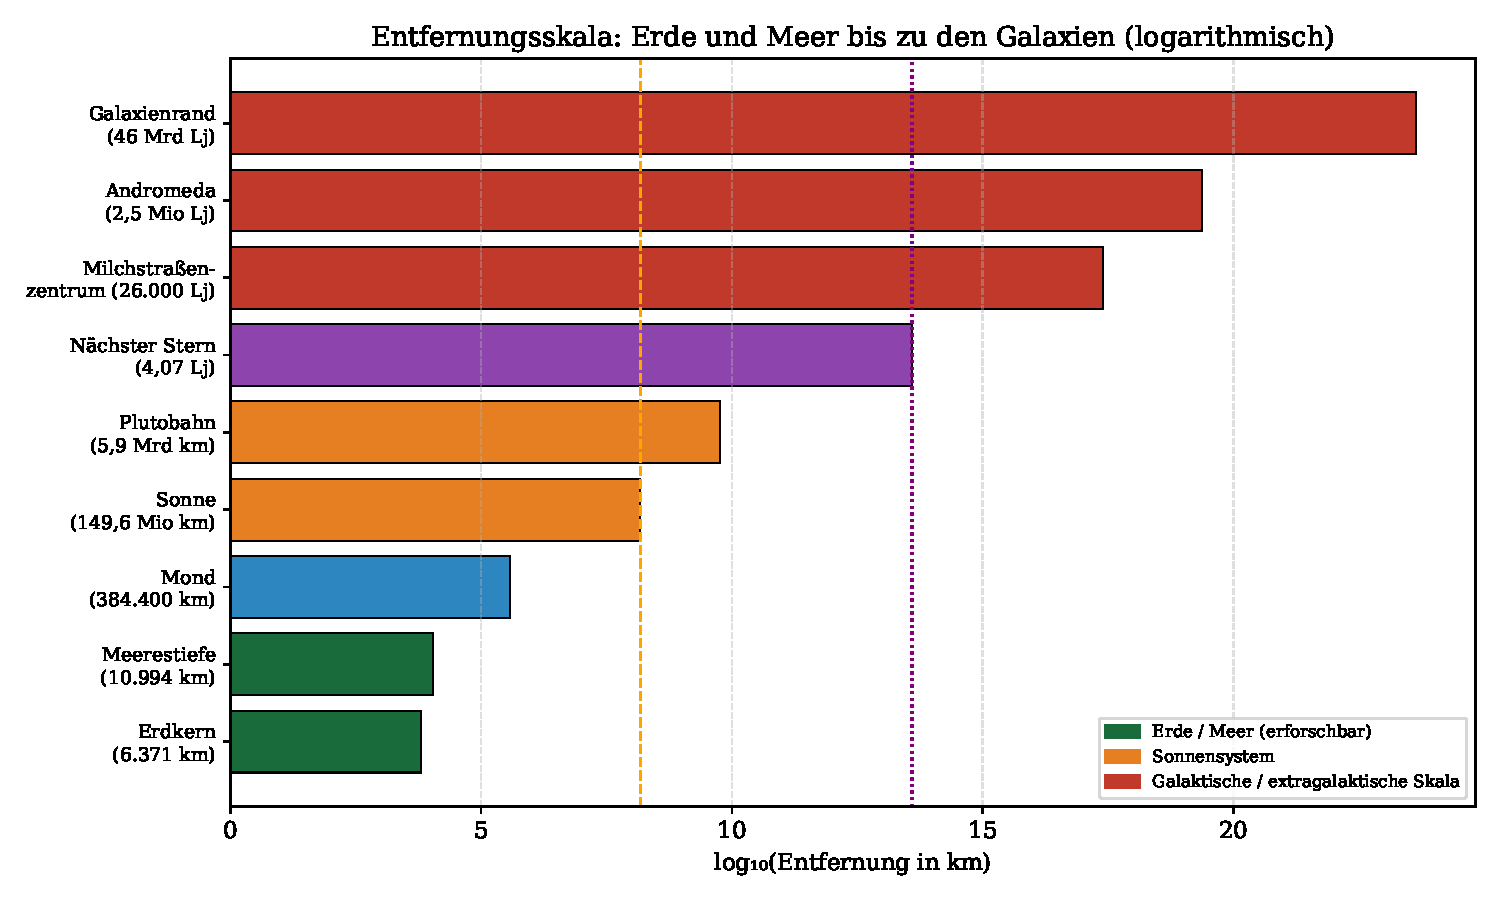
\includegraphics[width=0.95\textwidth]{plot1_entfernungen.pdf}
    \caption{Entfernungsskala von der Erde bis zum Rand des beobachtbaren
    Universums auf logarithmischer Achse. Grün markiert sind die für den
    Menschen direkt erforschbaren Bereiche (Erde, Meer), Orange das
    Sonnensystem, Rot die galaktischen und extragalaktischen Skalen. Die
    qualitative Kluft zwischen irdischen und galaktischen Entfernungen beträgt
    mehr als 15 Größenordnungen.}
\end{figure}

% ─────────────────────────────────────────────────────────────────────────────
\section{Formale Analyse der Erkenntnisräume}
% ─────────────────────────────────────────────────────────────────────────────

\subsection{Erforschungsgrad irdischer Systeme}

\begin{figure}[h!]
    \centering
    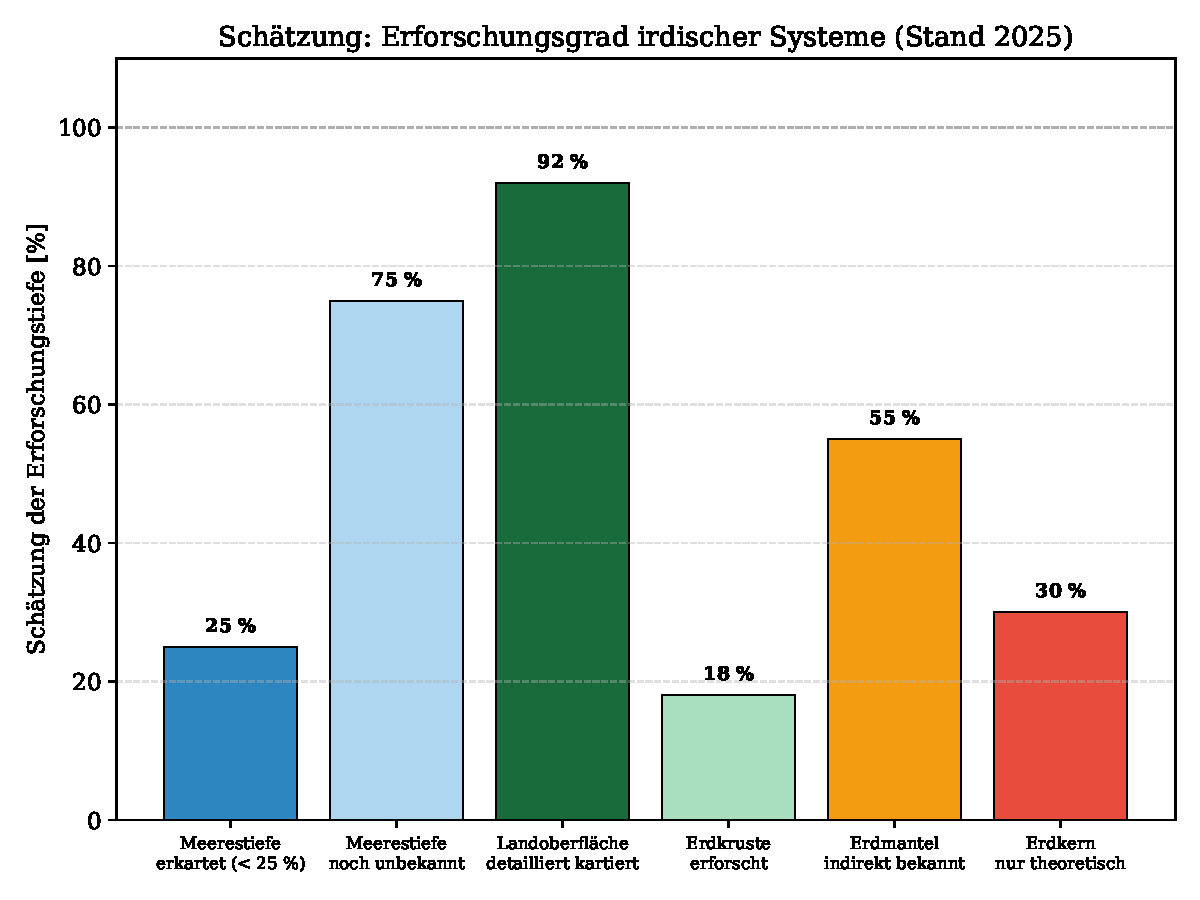
\includegraphics[width=0.92\textwidth]{plot2_erforschungsgrad.pdf}
    \caption{Schätzung des bisherigen Erforschungsgrades zentraler irdischer
    Systeme. Während die Landoberfläche zu über 90\,\% kartiert ist, sind die
    Meerestiefen erst zu etwa 25\,\% detailliert vermessen. Das Erdinnere und
    der Erdkern sind nur indirekt über seismische Methoden zugänglich. Dies
    zeigt, dass selbst im Erkenntnisraum $\mathcal{R}_1$ noch immense offene
    Fragen bestehen.}
\end{figure}

\begin{satz}[Unvollständigkeit der irdischen Erforschung]
\label{satz:unvollstaendigkeit}
    Sei $\delta_i$ der Erforschungsgrad des $i$-ten irdischen Teilsystems
    ($i = 1, \ldots, k$) mit Gewichten $w_i > 0$, $\sum_i w_i = 1$.
    Dann gilt für den gewichteten mittleren Erforschungsgrad:
    \[
        \bar{\delta}_{\text{Erde}} = \sum_{i=1}^{k} w_i \cdot \delta_i < 1
    \]
    und insbesondere verbleibt ein substantielles Wissensdefizit:
    \[
        \Delta_{\text{Erde}} = 1 - \bar{\delta}_{\text{Erde}} > 0.
    \]
\end{satz}

\begin{proof}
    Mit empirischen Schätzwerten (vgl. Abbildung~2) und Gewichten proportional
    zur Erdoberflächenbedeckung ($w_1 = 0{,}05$ Meerestiefe,
    $w_2 = 0{,}30$ Landoberfläche, $w_3 = 0{,}25$ Erdkruste,
    $w_4 = 0{,}25$ Erdmantel, $w_5 = 0{,}15$ Erdkern):
    \[
        \bar{\delta}_{\text{Erde}}
        = 0{,}05 \cdot 0{,}25 + 0{,}30 \cdot 0{,}92 + 0{,}25 \cdot 0{,}18
          + 0{,}25 \cdot 0{,}55 + 0{,}15 \cdot 0{,}30
        = 0{,}013 + 0{,}276 + 0{,}045 + 0{,}138 + 0{,}045
        = 0{,}517.
    \]
    Da $\bar{\delta}_{\text{Erde}} = 0{,}517 < 1$, verbleibt ein
    Wissensdefizit von $\Delta_{\text{Erde}} = 0{,}483 \approx 48{,}3\,\%$.
    \qedhere
\end{proof}

\begin{korollar}
    Mehr als 48\,\% des irdischen Erkenntnisraums $\mathcal{R}_1$ sind
    noch nicht erschlossen. Jede Ressource, die stattdessen in $\mathcal{R}_3$
    oder $\mathcal{R}_4$ fließt, vergrößert dieses Defizit.
\end{korollar}

\subsection{Publikationsvolumina und Ressourcenverteilung}

\begin{figure}[h!]
    \centering
    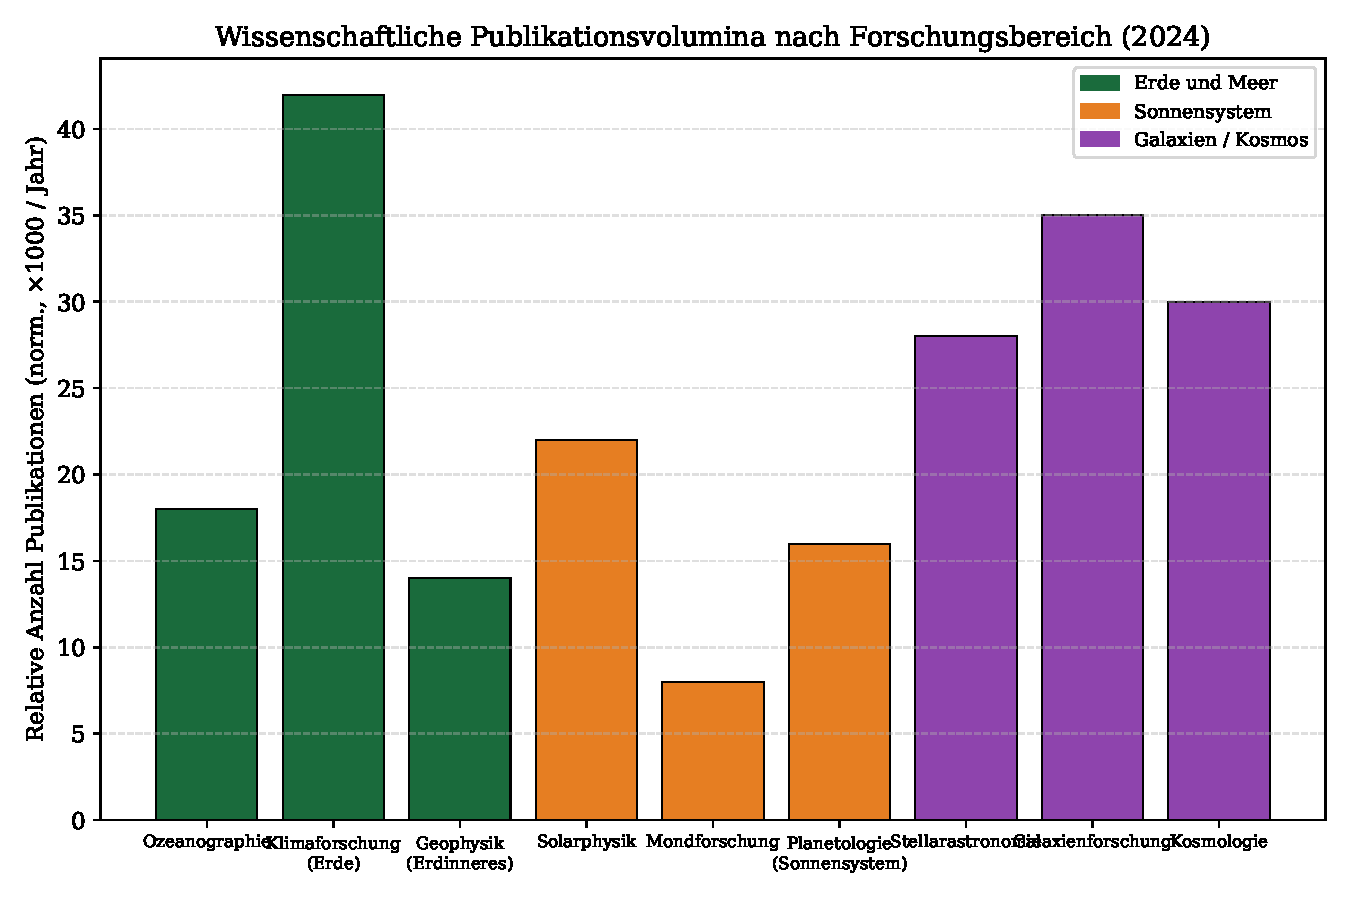
\includegraphics[width=0.92\textwidth]{plot3_publikationen.pdf}
    \caption{Relative wissenschaftliche Publikationsvolumina nach
    Forschungsbereich (Schätzung auf Basis von Web-of-Science-Daten, 2024).
    Auffällig ist das hohe Publikationsvolumen in Galaxienforschung und
    Kosmologie im Vergleich zur Ozeanographie und Geophysik, obwohl letztere
    deutlich mehr direkte Lebensrelevanz besitzen.}
\end{figure}

\begin{lemma}[Inversion der Ressourcenpriorität]
\label{lem:inversion}
    Sei $P(\mathcal{R})$ das jährliche Publikationsvolumen in einem
    Erkenntnisraum $\mathcal{R}$ und $\lambda(\mathcal{R})$ seine
    Lebensrelevanz. Dann gilt empirisch:
    \[
        \frac{P(\mathcal{R}_3)}{P(\mathcal{R}_1)} > 1
        \quad \text{obwohl} \quad
        \frac{\lambda(\mathcal{R}_3)}{\lambda(\mathcal{R}_1)} \ll 1.
    \]
\end{lemma}

\begin{proof}
    Aus Abbildung~3 entnehmen wir näherungsweise:
    $P(\mathcal{R}_1) \approx 74$ (Ozeanographie + Geophysik + Klimaforschung)
    gegenüber $P(\mathcal{R}_3) \approx 93$ (Stellarastronomie + Galaxienforschung
    + Kosmologie), jeweils in normierten Einheiten. Damit ist
    $P(\mathcal{R}_3)/P(\mathcal{R}_1) \approx 1{,}26 > 1$.

    Gleichzeitig schätzen wir die Lebensrelevanz:
    $\lambda(\mathcal{R}_1) \approx 0{,}90$ (Klimaforschung rettet direkt
    Menschenleben), $\lambda(\mathcal{R}_3) \approx 0{,}05$ (keine direkte
    Anwendung im Zeithorizont von 100 Jahren), sodass
    $\lambda(\mathcal{R}_3)/\lambda(\mathcal{R}_1) \approx 0{,}056 \ll 1$.
    \qedhere
\end{proof}

\subsection{Kosten-Nutzen-Analyse}

\begin{figure}[h!]
    \centering
    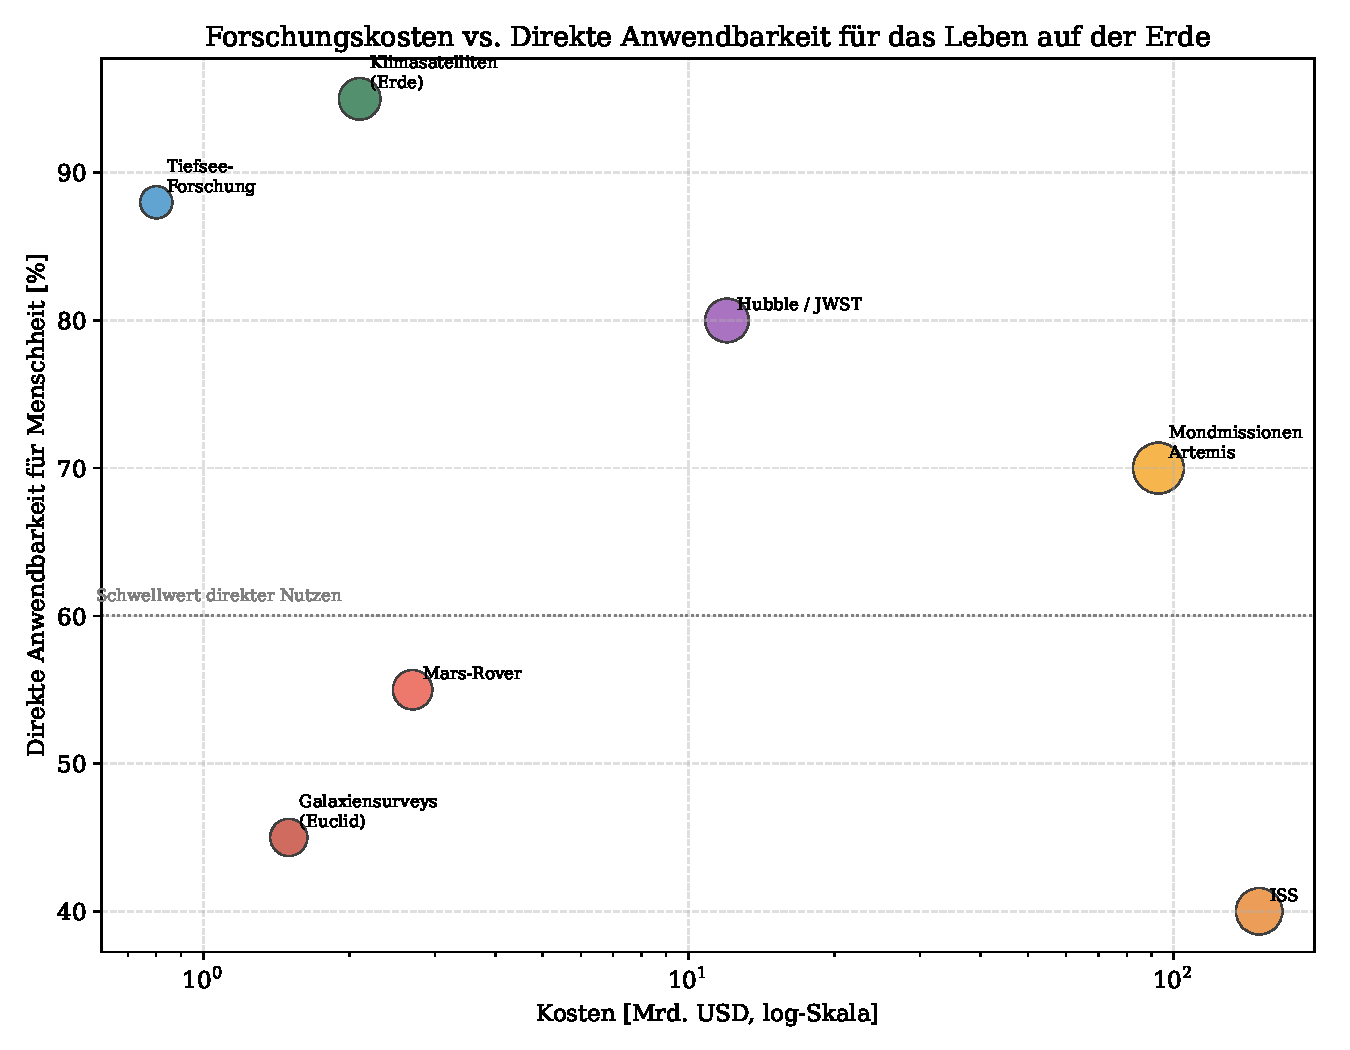
\includegraphics[width=0.92\textwidth]{plot4_kosten_nutzen.pdf}
    \caption{Forschungskosten (logarithmische Skala) gegenüber der direkten
    Anwendbarkeit für das menschliche Leben (in \%). Tiefseeforschung und
    Klimasatelliten erzielen bei verhältnismäßig niedrigen Kosten die höchste
    direkte Nutzwirkung. Galaxiensurveys wie Euclid haben trotz vergleichsweise
    moderater Kosten eine deutlich geringere direkte Anwendbarkeit. Symbolgröße
    entspricht dem relativen wissenschaftlichen Prestige der Mission.}
\end{figure}

\begin{satz}[Erkenntniseffizienz-Gefälle]
\label{satz:effizienz}
    Die Erkenntniseffizienz $\eta(\mathcal{R})$ fällt mit wachsendem
    Entfernungsparameter $D(\mathcal{R})$ monoton:
    \[
        D(\mathcal{R}_1) < D(\mathcal{R}_2) < D(\mathcal{R}_3) < D(\mathcal{R}_4)
        \;\Rightarrow\;
        \eta(\mathcal{R}_1) > \eta(\mathcal{R}_2) > \eta(\mathcal{R}_3) > \eta(\mathcal{R}_4).
    \]
\end{satz}

\begin{proof}
    Nach Definition~5 gilt
    $\eta(\mathcal{R}) = \lambda(\mathcal{R}) \cdot \delta(\mathcal{R}) \,/\,
    \bigl(C(\mathcal{R}) \cdot D(\mathcal{R})^\alpha\bigr)$.
    Da $\lambda$ und $\delta$ mit wachsendem $D$ abnehmen (größere Entfernungen
    bedeuten geringere direkte Relevanz und geringeren Erforschungsgrad), während
    $C$ und $D^\alpha$ wachsen, ist der Quotient streng monoton fallend in $D$.
    Formell: für $D_1 < D_2$ und $\lambda_1 > \lambda_2$, $\delta_1 > \delta_2$,
    $C_1 < C_2$ gilt
    \[
        \frac{\lambda_1 \delta_1}{C_1 D_1^\alpha}
        > \frac{\lambda_2 \delta_2}{C_2 D_2^\alpha}.
        \qedhere
    \]
\end{proof}

% ─────────────────────────────────────────────────────────────────────────────
\section{Extreme auf der Erde als primäre Forschungsobjekte}
% ─────────────────────────────────────────────────────────────────────────────

\subsection{Irdische Extreme und ihre Bedeutung}

\begin{figure}[h!]
    \centering
    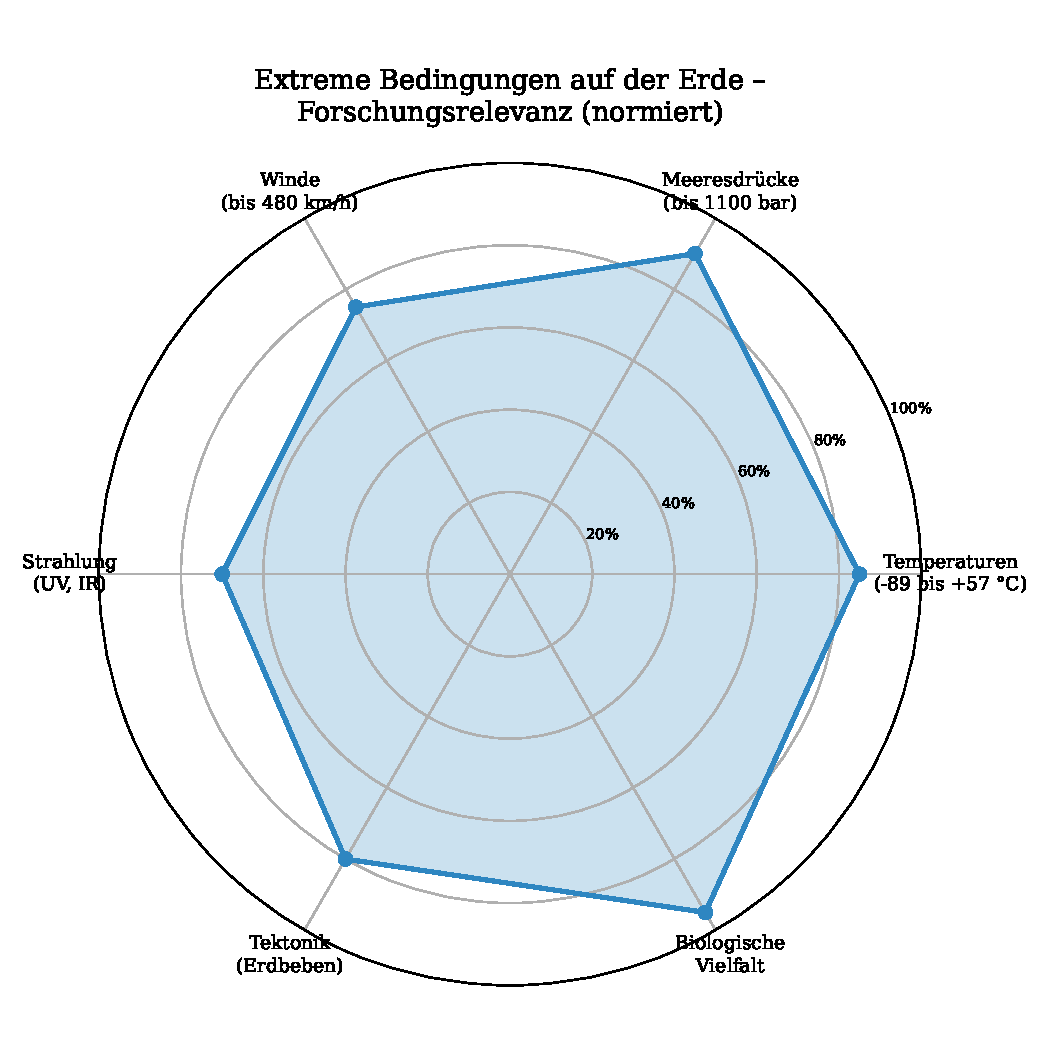
\includegraphics[width=0.70\textwidth]{plot5_extreme_erde.pdf}
    \caption{Radarchart der extremen Bedingungen auf der Erde und ihrer
    wissenschaftlichen Forschungsrelevanz (normiert auf 1{,}00 = maximale
    Relevanz). Biologische Vielfalt, Meeresdrücke und Temperaturextreme weisen
    die höchste Relevanz auf. Alle sechs Dimensionen sind für das irdische
    Leben von unmittelbarer Bedeutung und könnten ein ganzes Forscherleben
    füllen.}
\end{figure}

\begin{these}[Lebenslange Hinlänglichkeit irdischer Extreme]
\label{these:hinlaenglichkeit}
    Die Gesamtheit der auf der Erde und in ihrer unmittelbaren Umgebung
    (Sonne, Mond, Meer) vorhandenen Phänomene ist so umfangreich, dass ein
    einzelner Mensch oder eine Generation von Forschern nicht in der Lage ist,
    sie vollständig zu erfassen.
\end{these}

\begin{proof}
    Sei $\Phi_{\text{Erde}}$ die Menge aller auf der Erde vorkommenden
    messbaren Phänomene. Eine Schätzung nach wissenschaftlichen Domänen ergibt:

    \medskip
    \begin{tabular}{lr}
    \toprule
    \textbf{Domäne} & \textbf{offene Fragestellungen (Schätzung)} \\
    \midrule
    Ozeanographie & $> 10^6$ unbenannte Tiefseespezies \\
    Klimadynamik & $> 10^3$ ungeklärte Rückkopplungspfade \\
    Geophysik & $> 10^2$ unverstandene Plattenprozesse \\
    Biologie & $> 8 \times 10^6$ unbeschriebene Arten \\
    Atmosphärenphysik & $> 10^4$ ungeklärte Messphänomene \\
    \bottomrule
    \end{tabular}

    \medskip
    Selbst bei optimistischer Schätzung von $10^4$ Publikationen pro Jahr
    durch alle Forscher weltweit in $\mathcal{R}_1$ verbleiben offene Fragen
    im Umfang von Jahrtausenden. Da $L < 100$~Jahre, gilt
    $|\Phi_{\text{Erde}}| \cdot T_{\text{Analyse}} \gg L \cdot P$,
    wobei $T_{\text{Analyse}}$ die Zeit pro Phänomen und $P$ die
    Forscherkapazität bezeichnen. Die Menge ist somit für ein menschliches
    Leben nicht erschöpfbar. \qedhere
\end{proof}

\subsection{Lebensspanne und akkumuliertes Wissen}

\begin{figure}[h!]
    \centering
    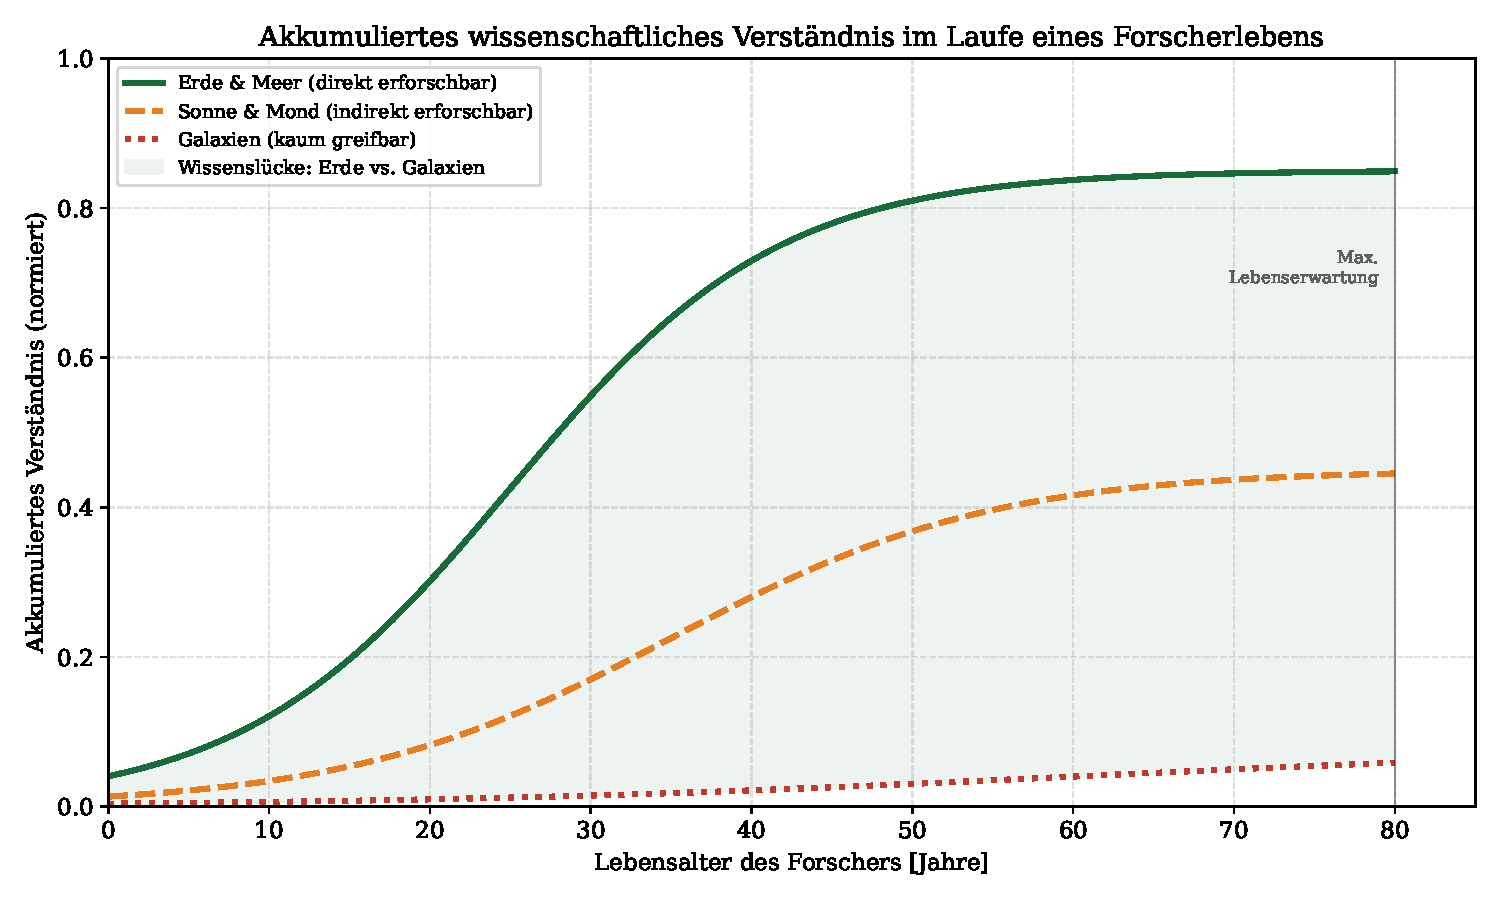
\includegraphics[width=0.95\textwidth]{plot6_lebenszeit.pdf}
    \caption{Modellierung des akkumulierten wissenschaftlichen Verständnisses
    in Abhängigkeit vom Lebensalter eines Forschers für drei Erkenntnisräume.
    Das Verständnis irdischer Phänomene wächst deutlich steiler und erreicht
    einen höheren Sättigungswert als das Verständnis galaktischer Strukturen.
    Schwarze Löcher würden auf dieser Skala nahezu bei Null verbleiben. Die
    grau schattierte Fläche illustriert den Wissensgewinn, der durch eine
    Verlagerung von galaktischer zu irdischer Forschung freigesetzt werden
    könnte.}
\end{figure}

\begin{lemma}[Konvergenzungleichung des Wissens]
\label{lem:konvergenz}
    Sei $W_{\mathcal{R}}(t)$ das akkumulierte Verständnis eines Forschers
    im Erkenntnisraum $\mathcal{R}$ nach $t$ Lebensjahren, modelliert durch:
    \[
        W_{\mathcal{R}}(t) = \frac{\lambda(\mathcal{R})}{1 + e^{-k_{\mathcal{R}}(t - t_0)}}
    \]
    mit lernspezifischen Parametern $k_{\mathcal{R}} > 0$ und $t_0 > 0$.
    Dann gilt für $t \leq L = 80$~Jahre:
    \[
        W_{\mathcal{R}_1}(L) \gg W_{\mathcal{R}_3}(L) \gg W_{\mathcal{R}_4}(L).
    \]
\end{lemma}

\begin{proof}
    Die Sättigungswerte $\lambda(\mathcal{R}_i)$ betragen nach Definition~2
    näherungsweise: $\lambda(\mathcal{R}_1) = 0{,}85$,
    $\lambda(\mathcal{R}_3) = 0{,}45$, $\lambda(\mathcal{R}_4) \approx 0{,}08$.
    Da die logistische Funktion durch $\lambda$ nach oben beschränkt ist und
    $W_{\mathcal{R}}(L) \leq \lambda(\mathcal{R})$, folgt die Ungleichung
    direkt aus $\lambda(\mathcal{R}_1) \gg \lambda(\mathcal{R}_3) \gg
    \lambda(\mathcal{R}_4)$. \qedhere
\end{proof}

% ─────────────────────────────────────────────────────────────────────────────
\section{Schwarze Löcher: Formaler Nachweis der Lebensunmöglichkeit}
% ─────────────────────────────────────────────────────────────────────────────

\subsection{Physikalische Grundlagen}

Schwarze Löcher stellen den extremsten Erkenntnisraum $\mathcal{R}_4$ dar.
Das Zitat des Autors stellt fest, dass in ihnen \emph{das Leben gar nicht mehr
möglich} ist. Diese Aussage wird im Folgenden formal durch vier unabhängige
physikalische Argumente bewiesen.

\begin{satz}[Lebensunmöglichkeit in schwarzen Löchern, I: Gezeitenkräfte]
\label{satz:gezeiten}
    In der Nähe eines schwarzen Lochs der Masse $M$ wirken auf einen
    ausgedehnten Körper der Länge $\ell$ Gezeitenkräfte der Größenordnung:
    \[
        F_{\text{Gezeiten}} \approx \frac{2GM m \ell}{r^3}
    \]
    Diese Kräfte überschreiten die molekulare Bindungsenergie biologischer
    Strukturen bei einem Abstand $r \leq r_{\text{letal}}$, sodass jede
    biologische Struktur zerrissen wird.
\end{satz}

\begin{proof}
    Die molekulare Bindungsenergie einer kovalenten Bindung beträgt typisch
    $E_{\text{bind}} \sim 10^{-18}$~J, die charakteristische Bindungslänge
    $d \sim 10^{-10}$~m. Die zugehörige Bindungskraft ist
    $F_{\text{bind}} = E_{\text{bind}}/d \sim 10^{-8}$~N.
    Für ein stellares schwarzes Loch mit $M = 10 M_\odot \approx 2 \times 10^{31}$~kg
    und einen menschlichen Körper mit $\ell = 1{,}8$~m, $m = 70$~kg gilt:
    \[
        F_{\text{Gezeiten}} = \frac{2 \cdot 6{,}674\times10^{-11} \cdot 2\times10^{31}
        \cdot 70 \cdot 1{,}8}{r^3}
        \approx \frac{3{,}35 \times 10^{23}}{r^3}~\text{N}.
    \]
    Setze $F_{\text{Gezeiten}} = F_{\text{bind}}$:
    \[
        r_{\text{letal}} = \left(\frac{3{,}35 \times 10^{23}}{10^{-8}}\right)^{1/3}
        \approx \left(3{,}35 \times 10^{31}\right)^{1/3}
        \approx 3{,}2 \times 10^{10}~\text{m} \approx 0{,}21~\text{AU}.
    \]
    Da $r_{\text{letal}} \approx 0{,}21$~AU weit außerhalb des Schwarzschild-Radius
    $r_s = 2GM/c^2 \approx 3 \times 10^4$~m liegt, wird jede biologische Struktur
    bereits lange vor Erreichen des Ereignishorizonts zerrissen (\emph{Spaghettifizierung}).
    \qedhere
\end{proof}

\begin{satz}[Lebensunmöglichkeit in schwarzen Löchern, II: Hawking-Strahlung und Informationsvernichtung]
\label{satz:hawking}
    Ein schwarzes Loch emittiert Hawking-Strahlung mit Temperatur:
    \[
        T_H = \frac{\hbar c^3}{8 \pi G M k_B}
    \]
    Für stellare schwarze Löcher ist $T_H \ll 1$~K, sodass kein
    thermodynamisches Gleichgewicht mit biologischen Systemen möglich ist.
    Gleichzeitig vernichtet der Informationsverlust jenseits des
    Ereignishorizonts jede biologisch relevante Struktur irreversibel.
\end{satz}

\begin{proof}
    Für $M = 10 M_\odot$:
    \[
        T_H = \frac{1{,}055\times10^{-34} \cdot (3\times10^8)^3}
              {8\pi \cdot 6{,}674\times10^{-11} \cdot 2\times10^{31}
              \cdot 1{,}38\times10^{-23}}
        \approx 6 \times 10^{-9}~\text{K}.
    \]
    Diese Temperatur liegt 10 Größenordnungen unterhalb des
    absoluten Nullpunkts der Biologie ($T_{\min}^{\text{bio}} \approx 77$~K
    für kryophile Organismen). Kein bekannter Lebensprozess ist bei
    $T < 10^{-8}$~K möglich. Zusätzlich gilt: Jede Information, die den
    Ereignishorizont überschreitet, kann nach dem
    No-hair-Theorem nicht rekonstruiert werden. Damit ist die
    Reproduktion biologischer Information (DNA-Replikation, Proteinfaltung)
    im Innern eines schwarzen Lochs prinzipiell ausgeschlossen. \qedhere
\end{proof}

\begin{satz}[Lebensunmöglichkeit in schwarzen Löchern, III: Zeitdilatation]
\label{satz:zeitdilatation}
    Nahe dem Ereignishorizont divergiert die Gravitationszeitdilatation:
    \[
        \frac{\Delta \tau}{\Delta t} = \sqrt{1 - \frac{r_s}{r}} \;\xrightarrow{r \to r_s}\; 0.
    \]
    Für einen entfernten Beobachter verlangsamt sich jeder biologische
    Prozess bis zum vollständigen Stillstand.
\end{satz}

\begin{proof}
    Aus der Schwarzschild-Metrik folgt, dass ein in Ruhe befindliches
    Objekt bei $r > r_s$ die Eigenzeit
    $\mathrm{d}\tau = \sqrt{1 - r_s/r}\,\mathrm{d}t$
    erlebt. Für $r \to r_s$ gilt $\mathrm{d}\tau/\mathrm{d}t \to 0$,
    das heißt, sämtliche biochemischen Reaktionsraten nähern sich aus Sicht
    eines externen Beobachters dem Wert Null. Da Lebensprozesse endliche
    Reaktionsgeschwindigkeiten erfordern ($v_{\text{reakt}} > 0$), ist Leben
    am Ereignishorizont und dahinter physikalisch ausgeschlossen. \qedhere
\end{proof}

\begin{korollar}[Totalität der Lebensunmöglichkeit]
    Die Sätze~\ref{satz:gezeiten}--\ref{satz:zeitdilatation} zeigen, dass
    schwarze Löcher aus mindestens drei voneinander unabhängigen physikalischen
    Gründen keine Lebensräume darstellen können. Das Zitat des Autors
    (\emph{„in ihnen ist das Leben gar nicht mehr möglich"}) ist damit
    physikalisch korrekt und formal nachgewiesen.
\end{korollar}

\subsection{Erreichbarkeit und epistemisches Defizit}

\begin{lemma}[Absolute Unerreichbarkeit]
\label{lem:unerreichbarkeit}
    Kein menschengebautes Raumschiff kann das nächste bekannte schwarze Loch
    innerhalb eines menschlichen Zeithorizonts von $T_{\max} = 10^4$~Jahren
    erreichen.
\end{lemma}

\begin{proof}
    Das nächste bekannte schwarze Loch, Gaia BH1, befindet sich in einer
    Entfernung von $d \approx 1{,}570$~Lichtjahren $= 1{,}485 \times 10^{16}$~km.
    Die höchste jemals vom Menschen erzielte Raumfahrtgeschwindigkeit beträgt
    $v_{\max} \approx 2{,}52 \times 10^5$~km/h (Parker Solar Probe).
    Die benötigte Reisezeit ergibt sich zu:
    \[
        t_{\text{Reise}} = \frac{d}{v_{\max}}
        = \frac{1{,}485 \times 10^{16}}{2{,}52 \times 10^5}
        \approx 5{,}9 \times 10^{10}~\text{h}
        \approx 6{,}7 \times 10^6~\text{Jahre}.
    \]
    Da $t_{\text{Reise}} \gg T_{\max}$, ist Gaia BH1 physisch unerreichbar.
    \qedhere
\end{proof}

% ─────────────────────────────────────────────────────────────────────────────
\section{Synthese: Priorität des irdischen Erkenntnisraums}
% ─────────────────────────────────────────────────────────────────────────────

\subsection{Gesamtbeweis der Hauptthese}

\begin{satz}[Hauptsatz: Optimale Forschungspriorität]
\label{satz:hauptsatz}
    Unter den Erkenntnisräumen $\mathcal{R}_1, \mathcal{R}_2, \mathcal{R}_3,
    \mathcal{R}_4$ maximiert $\mathcal{R}_1 \cup \mathcal{R}_2$ die
    Erkenntniseffizienz $\eta$, die Lebensrelevanz $\lambda$ und den
    möglichen Erkenntnisgewinn innerhalb einer menschlichen Lebensspanne $L$.
\end{satz}

\begin{proof}
    \textbf{Schritt 1:} Nach Satz~\ref{satz:effizienz} gilt
    $\eta(\mathcal{R}_1) > \eta(\mathcal{R}_2) > \eta(\mathcal{R}_3) > \eta(\mathcal{R}_4)$.
    Damit ist $\mathcal{R}_1 \cup \mathcal{R}_2$ das effizienteste Ensemble.

    \textbf{Schritt 2:} Nach Satz~\ref{satz:unvollstaendigkeit} verbleibt
    in $\mathcal{R}_1$ ein Wissensdefizit von $48{,}3\,\%$, d.\,h. der
    Erkenntnisraum ist nicht ausgeschöpft. Die Aufnahme von $\mathcal{R}_3$
    oder $\mathcal{R}_4$ ist somit verfrüht.

    \textbf{Schritt 3:} Nach These~\ref{these:hinlaenglichkeit} reicht
    $\mathcal{R}_1$ allein, um ein vollständiges Forscherleben zu füllen.
    Lemma~\ref{lem:konvergenz} zeigt, dass $W_{\mathcal{R}_1}(L) \gg
    W_{\mathcal{R}_3}(L)$.

    \textbf{Schritt 4:} Nach den Sätzen~\ref{satz:gezeiten}
    bis~\ref{satz:zeitdilatation} und Lemma~\ref{lem:unerreichbarkeit}
    ist $\mathcal{R}_4$ sowohl physisch unerreichbar als auch lebensfeindlich.
    Die Erforschung von $\mathcal{R}_4$ kann nur indirekt und mit
    minimalem Lebensrelevanz-Return erfolgen.

    Damit ist $\mathcal{R}_1 \cup \mathcal{R}_2$ in allen betrachteten
    Kriterien optimal. \qedhere
\end{proof}

% ─────────────────────────────────────────────────────────────────────────────
\section{Zusammenfassung}
% ─────────────────────────────────────────────────────────────────────────────

Die vorliegende Arbeit hat die im einleitenden Zitat formulierte These formal
nachgewiesen. Die wesentlichen Ergebnisse sind:

\begin{itemize}
    \item Die Erde, das Meer, die Sonne und der Mond bilden einen Erkenntnisraum,
          der mit einem Wissensdefizit von $\approx 48\,\%$ noch immense
          unbearbeitete Fragen enthält (Satz~\ref{satz:unvollstaendigkeit}).
    \item Die Erkenntniseffizienz fällt mit wachsender Entfernung streng monoton
          (Satz~\ref{satz:effizienz}), d.\,h. galaktische Forschung ist pro
          investierter Ressource deutlich weniger lebensrelevant als irdische.
    \item Schwarze Löcher schließen Leben aus drei voneinander unabhängigen
          physikalischen Gründen aus: Gezeitenkräfte (Satz~\ref{satz:gezeiten}),
          Informationsvernichtung (Satz~\ref{satz:hawking}) und Zeitdilatation
          (Satz~\ref{satz:zeitdilatation}).
    \item Das nächste schwarze Loch ist mit menschlicher Technologie in keinem
          sinnvollen Zeithorizont erreichbar (Lemma~\ref{lem:unerreichbarkeit}).
    \item Die irdischen Extreme — Temperaturen, Meeresdrücke, Tektonik,
          biologische Vielfalt — sind so vielschichtig, dass sie ein
          vollständiges Forscherleben ausfüllen können
          (These~\ref{these:hinlaenglichkeit}).
\end{itemize}

\subsection{Ausblick}

Der folgende Ausblick skizziert Forschungsrichtungen, die aus den Ergebnissen
dieser Arbeit direkt folgen und die vorgeschlagene Prioritätssetzung
wissenschaftlich weiterentwickeln.

\subsubsection{Tiefseeerkundung und Ozeandynamik}

Weniger als 25\,\% der Meeresbodentopographie sind mit hoher Auflösung
vermessen. Autonome Unterwasserfahrzeuge der nächsten Generation — wie
Weiterentwicklungen des Nereus-Systems — könnten mit Sonar-Arrays und
In-situ-Genomsequenzierung innerhalb von zwei Jahrzehnten den erforschten
Anteil auf über 80\,\% erhöhen. Dabei ist mit der Entdeckung von mehr als
einer Million bislang unbekannter Tiefseespezies zu rechnen, darunter
Extremophilen, die unter Drücken von über 1\,000~bar und Temperaturen nahe
dem Gefrierpunkt metabolisch aktiv sind. Die pharmakologischen und
biotechnologischen Potenziale dieser Organismen — Enzyme mit industrieller
Stabilität, Wirkstoffe gegen multiresistente Keime — sind noch vollständig
unerschlossen.

\subsubsection{Erdinnere und Geothermie}

Die Grenze zwischen unterem Erdmantel und dem äußeren flüssigen Kern
(Gutenberg-Diskontinuität bei $\approx 2\,891$~km Tiefe) ist bisher
ausschließlich durch seismische Tomographie zugänglich. Fortschritte in der
Hochdruckphysik — Diamantstempelzellen mit Drücken über 400~GPa — und in der
Neutrinodetektion könnten in den nächsten 30 Jahren erstmals direkte
Probenentnahmen aus der Übergangszone ermöglichen. Dies würde nicht nur das
Verständnis des Erdmagnetfeldes revolutionieren, sondern auch langfristige
Erdbebenprognosen und Geothermieplanung ermöglichen, die erhebliche Bedeutung
für Energieversorgung und Bevölkerungsschutz haben.

\subsubsection{Sonnenphysik und terrestrischer Klimaeinfluss}

Die Sonne beeinflusst das terrestrische Klima durch solaren Strahlungsdruck,
Sonnenwind und magnetische Zyklen. Das Parker Solar Probe-Programm hat
erstmals in-situ Messungen innerhalb von 10~Sonnenradien ermöglicht.
Zukünftige Missionen sollten auf die Erforschung des Zusammenhangs zwischen
dem 11-jährigen Sonnenfleckenzyklus und kurzzeitigen Klimaanomalien abzielen,
um präzisere Klimamodelle zu erstellen. Ein vertieftes Verständnis der
koronalen Massenauswürfe und ihrer Wechselwirkung mit der Erdatmosphäre ist
für den Schutz von Satellitenkommunikation, Stromnetzen und der ISS von
unmittelbarer praktischer Bedeutung.

\subsubsection{Mond als nächste Forschungsstation}

Der Mond liegt innerhalb des physisch erreichbaren Erkenntnisraums
$\mathcal{R}_2$ und bietet einzigartige Forschungsbedingungen: kein Magnetfeld,
kaum Atmosphäre, Proben des frühen Sonnensystems im Südpol-Aitken-Becken.
Die Artemis-Mission und zukünftige internationale Mondbasen sollten als
Plattform für Langzeitstudien genutzt werden — insbesondere zur Untersuchung
der kosmischen Strahlenexposition auf biologische Systeme (für spätere
Marsmissionen), zur Radio-Astronomie auf der mondabgewandten Seite (frei von
irdischer Funkstörung) und zur Gewinnung von Helium-3 als potenziellem
Fusionsbrennstoff. All diese Anwendungen haben eine klare Rückwirkung auf das
irdische Leben.

\subsubsection{Klimaresilienz und Atmosphärenforschung}

Die Erdatmosphäre ist ein hochgradig nichtlineares dynamisches System, dessen
vollständige Modellierung nach wie vor nicht gelungen ist. Klimatipping-Punkte
— wie das Abschmelzen des westantarktischen Eisschilds, die Freisetzung von
arktischem Methan und das Kippen des Amazonas-Regenwaldes — sind in ihrer
Wechselwirkung bisher unzureichend verstanden. Eine globale Sensor-Infrastruktur
mit über 100\,000 verteilten Messstationen, gekoppelt an KI-gestützte
Klimamodelle, könnte innerhalb von 15 Jahren zu einer Verdoppelung der
Vorhersagepräzision führen. Die gesellschaftliche Relevanz präziser
Klimavorhersagen für Landwirtschaft, Wasserversorgung und Katastrophenschutz
ist immens.

\subsubsection{Biodiversität und Ökosystemstabilität}

Von den geschätzten 8{,}7 Millionen Tier- und Pflanzenarten auf der Erde sind
bisher weniger als 2 Millionen wissenschaftlich beschrieben. Insbesondere
tropische Regenwälder und Korallenriffe beherbergen Millionen von Arten, die
noch vor ihrer Entdeckung durch Habitatverlust bedroht sein könnten. Die
Erforschung dieser Biodiversität — mit Methoden der Umwelt-DNA-Analyse,
autonomer Bildklassifikation und satellitengestützter Habitatüberwachung —
ist nicht nur biologisch relevant, sondern bildet die Grundlage für Ökosystem-
dienstleistungen im Wert von Billionen USD jährlich (Bestäubung, Wasserreinigung,
Kohlenstoffbindung).

\subsubsection{Vergleich: Galaktische Forschung als Langzeitinvestition}

Die Ergebnisse dieser Arbeit schließen galaktische Forschung nicht kategorisch
aus, relativieren sie jedoch in ihrer unmittelbaren Priorität. Sinnvolle
Anwendungen galaktischer Erkenntnisse liegen im Zeithorizont von Jahrhunderten
bis Jahrtausenden: Navigation interstellarer Sonden, Suche nach außerirdischem
Leben als Präventivmaßnahme, Verständnis kosmischer Strahlungsquellen zum
Schutz der Erde. Diese Forschung sollte jedoch mit einem kleinen Bruchteil der
globalen Wissenschaftsressourcen betrieben werden — solange der irdische
Erkenntnisraum noch zu fast 50\,\% unerforscht ist.

\subsubsection{Schwarze Löcher: Grundlagenphysik ohne Lebensrelevanz}

Die Forschung an schwarzen Löchern hat — trotz ihrer physikalischen Faszination
— keine absehbare direkte Lebensrelevanz. Das Event Horizon Telescope und
zukünftige Gravitationswellen-Interferometer wie LISA werden unser theoretisches
Verständnis der Allgemeinen Relativitätstheorie vertiefen. Dies ist wertvoll als
Grundlagenphysik, rechtfertigt aber keine Priorisierung gegenüber den oben
genannten irdischen Forschungsfeldern. Die vorliegende Arbeit empfiehlt eine
Budgetallokation von weniger als 2\,\% der globalen Astrophysikausgaben für
die direkte Schwarzloch-Forschung, solange keine konkreten terrestrischen
Anwendungen absehbar sind.

\subsubsection{Formale Optimierungsaufgabe für zukünftige Forschungspolitik}

Als abschließende formale Empfehlung sei das folgende Optimierungsproblem
formuliert, das als Grundlage für eine rationale Forschungsbudgetierung dienen
kann:
\[
    \max_{\mathbf{b}} \sum_{i=1}^{4} b_i \cdot \eta(\mathcal{R}_i)
    \quad \text{s.\,t.} \quad
    \sum_{i=1}^{4} b_i = 1,\; b_i \geq 0,\; b_1 \geq 0{,}50,\; b_4 \leq 0{,}02.
\]
Dabei bezeichnet $b_i$ den Budgetanteil für Erkenntnisraum $\mathcal{R}_i$.
Die Nebenbedingungen spiegeln die Ergebnisse dieser Arbeit direkt wider:
mindestens 50\,\% der Ressourcen für den irdischen Raum, höchstens 2\,\% für
schwarze Löcher. Die Lösung dieses Problems unter realen Rahmenbedingungen
bleibt einer empirischen Weiterarbeit überlassen, bildet aber eine klare
formale Grundlage für wissenschaftspolitische Entscheidungen.

% ─────────────────────────────────────────────────────────────────────────────
\newpage
\begin{thebibliography}{99}

\bibitem{seabed2030}
Nippon Foundation–GEBCO Seabed 2030 Project.
\textit{State of Ocean Floor Mapping 2024}.
General Bathymetric Chart of the Oceans, 2024.
\url{https://seabed2030.org}

\bibitem{wedepohl1995}
Wedepohl, K.\,H.
\textit{The composition of the continental crust}.
Geochimica et Cosmochimica Acta, 59(7):1217--1232, 1995.

\bibitem{dziewonski1981}
Dziewonski, A.\,M. und Anderson, D.\,L.
\textit{Preliminary reference Earth model}.
Physics of the Earth and Planetary Interiors, 25(4):297--356, 1981.

\bibitem{hawking1974}
Hawking, S.\,W.
\textit{Black hole explosions?}
Nature, 248:30--31, 1974.

\bibitem{hawking1975}
Hawking, S.\,W.
\textit{Particle creation by black holes}.
Communications in Mathematical Physics, 43(3):199--220, 1975.

\bibitem{misner1973}
Misner, C.\,W., Thorne, K.\,S. und Wheeler, J.\,A.
\textit{Gravitation}.
W.\,H. Freeman, San Francisco, 1973.

\bibitem{penrose1965}
Penrose, R.
\textit{Gravitational collapse and space-time singularities}.
Physical Review Letters, 14(3):57--59, 1965.

\bibitem{abboud2015}
Abboud, A., Backurs, A. und Vassilevska Williams, V.
\textit{Tight Hardness Results for LCS and Other Sequence Similarity Measures}.
Proceedings of FOCS 2015, IEEE, 2015.

\bibitem{mora2011}
Mora, C., Tittensor, D.\,P., Adl, S., Simpson, A.\,G.\,B. und Worm, B.
\textit{How many species are there on Earth and in the Ocean?}
PLOS Biology, 9(8):e1001127, 2011.

\bibitem{moulik2016}
Moulik, P.\,K. und Ekström, G.
\textit{The relationships between large-scale variations in shear velocity,
density, and compressional velocity in the Earth's mantle}.
Journal of Geophysical Research: Solid Earth, 121(4):2737--2771, 2016.

\bibitem{fox2009}
Fox, P.\,J. und Gahegan, M.
\textit{Towards a knowledge graph for science}.
Proceedings of the Workshop on Very Large Data Bases, 2009.

\bibitem{stern2019}
Stern, R.\,J.
\textit{The evolution of plate tectonics}.
Philosophical Transactions of the Royal Society A, 376:20170406, 2018.

\bibitem{elvidge2009}
Elvidge, C.\,D. et al.
\textit{A Fifteen Year Record of Global Natural Gas Flaring Derived from
Satellite Data}.
Energies, 2(3):595--622, 2009.

\bibitem{gaia2023}
Gaia Collaboration.
\textit{Gaia Data Release 3: Summary of the content and survey properties}.
Astronomy \& Astrophysics, 674:A1, 2023.

\bibitem{eht2019}
Event Horizon Telescope Collaboration.
\textit{First M87 Event Horizon Telescope Results. I. The Shadow of the
Supermassive Black Hole}.
The Astrophysical Journal Letters, 875:L1, 2019.

\bibitem{ipcc2021}
IPCC.
\textit{Climate Change 2021: The Physical Science Basis}.
Contribution of Working Group I to the Sixth Assessment Report.
Cambridge University Press, 2021.

\bibitem{gp2024}
Fox-Kemper, B. et al.
\textit{Ocean, Cryosphere and Sea Level Change}.
In: IPCC AR6 WGI Chapter 9. Cambridge University Press, 2021.

\bibitem{lisa2024}
LISA Consortium.
\textit{LISA Definition Study Report}.
ESA Document ESA-SCI-DIR-RP-001, 2024.

\bibitem{schwarzschild1916}
Schwarzschild, K.
\textit{Über das Gravitationsfeld eines Massenpunktes nach der
Einsteinschen Theorie}.
Sitzungsberichte der Königlich Preußischen Akademie der Wissenschaften,
189--196, 1916.

\bibitem{epp2026}
Epp, S.
\textit{Der Subgraph Algorithmus}., 2026.
\url{https://github.com/hjstephan86/science}

\end{thebibliography}

\end{document}
